%% ===================== PREAMBLE =====================
\documentclass[11pt]{article}
\usepackage[utf8]{inputenc}
\usepackage[T1]{fontenc}
\usepackage{lmodern}
\usepackage[letterpaper,margin=1in]{geometry}
\usepackage{amsmath,amssymb,mathtools}
\usepackage{graphicx}
\usepackage{booktabs}
\usepackage{tabularx}
\usepackage{caption}
\usepackage{float}
\usepackage{enumitem}
\usepackage{xcolor}
\usepackage{microtype}
\usepackage{setspace}
\usepackage[colorlinks=true,linkcolor=black,citecolor=black,urlcolor=blue!55!black]{hyperref}
\hypersetup{
  pdftitle={Incremental predictive value of a spectral fragility index for atrial
            reentry: a pre-registered in-silico evaluation with a clinical
            recurrence endpoint},
  pdfauthor={Mounish Mavuduru},
  pdfsubject={Original Investigation submitted to JAMA Cardiology},
  pdfkeywords={atrial fibrillation; reentry; biomarker; prediction model;
               spectral graph theory; algebraic connectivity; negative result;
               pre-registration; TRIPOD+AI}
}
\graphicspath{{figures/}}
\newcommand{\lam}{\lambda}
\newcommand{\phii}{\varphi}
\newcommand{\rhoval}{\rho}
\newcommand{\SFI}{\ensuremath{\mathrm{SFI}}}
\newcommand{\dAUC}{\ensuremath{\Delta\mathrm{AUC}}}
\newcommand{\code}[1]{\texttt{#1}}
\emergencystretch=2em
\hbadness=2500
\captionsetup{font=small,labelfont=bf}

%% ===================== TITLE PAGE =====================
\begin{document}
\thispagestyle{empty}

\begin{center}
{\Large\bfseries Incremental predictive value of a spectral fragility index for
atrial reentry: a pre-registered in-silico evaluation with a clinical
recurrence endpoint\par}
\end{center}

\vspace{0.7em}
\noindent\textbf{Running title.} SPECTRAL FRAGILITY INDEX FOR ATRIAL REENTRY

\smallskip
\noindent\textbf{Article type.} Original Investigation. \textbf{Study type.}
Diagnostic/Prognostic Study.

\smallskip
\noindent\textbf{Author.} Mounish Mavuduru

\smallskip
\noindent\textbf{Affiliation.} Independent researcher (unaffiliated).

\smallskip
\noindent\textbf{ORCID.} 0009-0009-4102-6075

\smallskip
\noindent\textbf{Corresponding author.} Mounish Mavuduru, 4912 Spanish Oaks Dr,
McKinney, TX 75070, USA. Telephone (+1) 945-527-6483. E-mail:
\href{mailto:mounishmavuduru@gmail.com}{mounishmavuduru@gmail.com}

\vspace{0.7em}
\noindent\textbf{Reporting guideline.} TRIPOD+AI, for the clinical endpoint;
completed checklist in Supplement~1.

\smallskip
\noindent\textbf{Scope.} Computational (in-silico) study. All ground-truth labels
are electrophysiology-simulator inducibility verdicts with a single exception:
the pre-registered clinical endpoint, scored against real two-year
post-ablation arrhythmia recurrence in the $82$ University of Washington
patients. No post-operative atrial fibrillation outcome was simulated.

\vspace{0.7em}
\noindent\textbf{Word count, tables and figures}

\smallskip
\begin{tabular}{@{}ll@{}}
\toprule
Word count (main text)  & 2930 \\
Word count (abstract)   & 350 \\
Key Points              & 97 \\
Tables and figures      & 5 (2 tables, 3 figures) \\
References              & 19 \\
Online-only material    & Supplement 1, Supplement 2 \\
\bottomrule
\end{tabular}

\newpage

%% ===================== KEY POINTS =====================
\noindent\textbf{Key Points}

\paragraph{Question.} Does a graph-spectral fragility index (\SFI) computed from
patient-derived left-atrial meshes improve prediction of simulated reentry
inducibility beyond published competitor features?

\paragraph{Findings.} In a pre-registered evaluation of $182$ patient-derived
left-atrial meshes, the incremental $\dAUC$ for simulator-determined reentry
inducibility was $+0.012$ (bootstrap interval, $-0.017$ to $+0.044$), excluding
the pre-registered $0.05$ threshold; the primary endpoint was not met. A
pre-registered clinical endpoint in $82$ patients was also not met.

\paragraph{Meaning.} The index added nothing beyond established fibrosis and
connectivity features. The interval excludes the pre-specified effect size, so
the study measured the effect rather than failing to detect it.

\newpage

%% ===================== ABSTRACT =====================
\section*{Abstract}
\noindent\textbf{Importance.} Algebraic connectivity $\lam_2$ and its
closed-form per-edge sensitivity govern stability in coupled excitable networks,
motivating a biomarker of atrial reentry that aggregates that sensitivity over a
fibrosis-weighted conduction-uncoupling field. Whether it adds information
beyond established fibrosis and connectivity features was unknown.

\medskip
\noindent\textbf{Objective.} To determine, under a protocol pre-registered
before any label was inspected, whether the Spectral Fragility Index (\SFI)
adds incremental discrimination for atrial reentry beyond published features.

\medskip
\noindent\textbf{Design, Setting, and Participants.} Pre-registered in-silico
evaluation on $182$ patient-derived left-atrial meshes from two
de-identified public deposits (Roney virtual cohort, $n=100$; University of Washington
late-gadolinium-enhancement cohort, $n=82$; no attrition) and up to $100{,}000$
synthetic excitable networks, with a pre-registered clinical arm in those $82$
patients, all followed two years after ablation.

\medskip
\noindent\textbf{Exposures.} \SFI, computed from pre-ablation anatomy and
entered only as an add-on to six competitor features (fibrosis burden, spatial
entropy, patch size, minimum cut, percolation threshold, $\lam_2$).

\medskip
\noindent\textbf{Main Outcomes and Measures.} In-silico, a simulator's
reentry-inducibility verdict, not clinical atrial fibrillation; clinically,
two-year post-ablation arrhythmia recurrence. Penalised logistic regression and
gradient-boosted trees were fitted under patient- and shape-family-held-out
\code{GroupKFold} and compared by paired DeLong test with $\geq10^{4}$ bootstrap
resamples. The primary endpoint required grouped $\dAUC\geq0.05$ with $p<0.05$;
the clinical arm pre-specified a minimum detectable $\dAUC$ of $0.10$--$0.15$
and fixed-sequence stopping.

\medskip
\noindent\textbf{Results.} The primary endpoint was not met. Across the combined
real cohorts ($42$ inducible of $182$), gradient boosting gave $\dAUC=+0.012$
(bootstrap CI $[-0.017,+0.044]$; $p=0.449$), excluding the $0.05$ threshold, so
power was not the limiting factor; synthetic-network $\dAUC$ converged to
$+0.003$. The clinical gate fired ($\dAUC=+0.197$; $p=0.0061$), but the plan
frozen before outcomes were joined identified an artefact of an anti-predictive
baseline (AUC $0.250$) that nine columns of Gaussian noise reproduced (empirical
$p=0.333$); that endpoint was not met and testing halted. \SFI\ aggregates were
reconstructible from the competitors ($R^{2}=0.970$), an exact-recompute variant
added nothing, and the estimator was ill-conditioned on real tissue (median
$\rhoval\approx2422$; limit $\rhoval^{\ast}\approx3$).

\medskip
\noindent\textbf{Conclusions and Relevance.} \SFI\ added no practically
meaningful predictive value for atrial reentry beyond existing features, and its
one nominally positive patient-outcome result was a false positive its own
pre-registered guards caught. These findings do not support clinical use.

\newpage

%% ===================== MAIN TEXT =====================
\section{Introduction}
Atrial fibrillation is sustained on a remodelled conduction substrate.
Interstitial fibrosis slows and disorganises propagation, and the resulting
wavelength shortening, source--sink mismatch, and unidirectional block permit
reentry. Because that substrate is a network of coupled excitable elements,
graph-theoretic and spectral summaries of the atrial conduction network have
been proposed as substrate biomarkers. One such summary is algebraic
connectivity $\lam_2$, the second-smallest Laplacian eigenvalue (Fiedler,
1973)~\cite{fiedler1973}. It governs the stability of synchronised states in
coupled excitable and oscillator networks through the master-stability function
(Pecora and Carroll, 1998)~\cite{pecora1998} and the synchronizability
eigenratio $\lam_N/\lam_2$~\cite{barahona2002}, and it has been fielded as a
real-time seizure detector~\cite{bomela2020}. Its sensitivity to a single
conduction weight has a classical closed form,
$\partial\lam_2/\partial w_{ij}=(\phii_{2,i}-\phii_{2,j})^2$ (Ghosh and Boyd,
2006)~\cite{ghosh2006}, where $\phii_2$ is the Fiedler vector. Aggregating that
sensitivity over a fibrosis-weighted conduction-uncoupling field yields a
per-region Spectral Fragility Index (SFI).

Whether such an index carries information beyond the substrate features already
in use has not been established. Fibrosis burden, fibrosis spatial
heterogeneity, fibrosis patch size, and connectivity measures such as the global
minimum cut, the percolation threshold, and $\lam_2$ itself are computed from
the same meshes at negligible cost. A spectral index earns a place beside them
only if it improves discrimination when added to them, by a margin fixed in
advance as the one that would matter, under cross-validation that holds out
whole patients and shape families so anatomy cannot leak between training and
test folds. Evaluations imposing all of this at once have not been reported.

This study evaluated SFI as a strict add-on to six competitor features,
predicting simulator reentry inducibility in $182$ patient-derived left-atrial
meshes ($100$ Roney~\cite{roney2022}, $82$ University of
Washington~\cite{uwboyle2025}) and in up to $100{,}000$ synthetic excitable
networks. A pre-registered clinical endpoint followed: two-year post-ablation
arrhythmia recurrence in the $82$ University of Washington patients. The
endpoints, cross-validation scheme, baseline feature set, effect-size threshold
($\dAUC\geq 0.05$), and the accepted null that SFI merely re-encodes fibrosis
were frozen before any label was inspected.

\section{Methods}

\paragraph{Design and pre-registration.} The endpoints, cross-validation scheme,
baseline feature set, and the accepted null were frozen and git-tagged before any
label was inspected. The null hypothesis that SFI merely re-encodes fibrosis was
pre-registered as an accepted, reportable outcome. The section of the
pre-registration governing the clinical analysis was frozen before any feature was
placed beside the outcome column; that analysis was run once and is reported as it
came out.

\paragraph{Reporting guideline.} One analysis here is scored against a real
patient outcome: prediction of two-year post-ablation arrhythmia recurrence in
the $82$ University of Washington (UW) patients. That endpoint
is reported in accordance with TRIPOD+AI~\cite{tripodai2024}, and a completed checklist accompanies
this article. Adherence is claimed for that endpoint alone. Every other outcome
here is an electrophysiology simulator's verdict on reentry inducibility, which
falls outside the statement's remit, though those analyses follow the same
frozen protocol.

\paragraph{Cohorts.} Two public patient-derived left-atrial mesh deposits were
used. The Roney virtual cohort~\cite{roney2022} (Zenodo 5801337) contains $100$ meshes and all
$100$ were analysed; fibrosis is a continuous fraction mapped from the shipped
image-intensity ratio~\cite{khurram2014}. The UW/Boyle late-gadolinium-enhancement cohort~\cite{uwboyle2025} (Dryad
\code{10.5061/dryad.kkwh70sg0}) contains $164$ meshes, being $82$ patients imaged
before and after ablation; the primary analysis used the $82$ pre-ablation meshes
only, because post-ablation geometry encodes the delivered treatment. That
release ships no intensity ratios (withheld under its institutional review
board), so its fibrosis was derived from the per-element tissue tags and is
two-valued. No subject was excluded for any other reason, giving $182$ analysed
meshes with no attrition. Both deposits are de-identified and carry anatomy only,
with no age, sex, race, ethnicity, or comorbidity variables. The per-patient
two-year recurrence outcomes were supplied on request by the UW cohort's authors,
who confirmed they carry no confidentiality restriction. Synthetic excitable
networks (up to $100{,}000$ random geometric graphs) were used only for the scale
behaviour of the null and for cross-medium transfer.

\paragraph{Conduction graph and index.} Nodes were mesh vertices and edges
triangle edges, with weight
$w_{ij}=[c_\perp+(c_\parallel-c_\perp)a_{ij}^{2}]\cdot\mathrm{clip}(1-\phi_{ij},\varepsilon,1)$,
where $a_{ij}$ is edge--fibre alignment, $\phi_{ij}$ mean endpoint fibrosis,
$c_\parallel=1.0$, $c_\perp=0.3$, and $\varepsilon=0.05$; $L=D-W$ has algebraic
connectivity $\lam_2$ with Fiedler vector $\phii_2$. Diffuse fibrosis-weighted
uncoupling $\Delta w$ (mean $\Delta w\approx0.36$, frozen in the pre-registration)
gives, to first order,
\begin{equation}
\SFI(R)\;\approx\;\sum_{(i,j)\in R}\mathbb{E}[\Delta w_{ij}]\,
(\phii_{2,i}-\phii_{2,j})^{2},
\qquad
\frac{\partial\lam_2}{\partial w_{ij}}=(\phii_{2,i}-\phii_{2,j})^{2},
\end{equation}
a classical identity. First-order, basis-independent subspace, and
exact-recompute variants were all computed on $\sim\!2000$-node coarsened graphs.

\paragraph{Comparator features and outcomes.} SFI was evaluated strictly as an
add-on to six published competitor features it had to beat: fibrosis burden,
fibrosis spatial entropy, fibrosis patch size, deterministic global min-cut
(Stoer--Wagner), percolation threshold, and $\lam_2$ alone. The in-silico outcome
was a monodomain Mitchell--Schaeffer~\cite{mitchell2003} inducibility verdict (self-sustained reentry
$\geq650$~ms after burst pacing at a cycle length of $150$~ms from random sites),
$42$ of $182$ meshes inducible; this is a simulator verdict and not clinical
atrial fibrillation. Clinically, the outcome was recurrence, defined as at least
$30$ seconds of documented atrial fibrillation or flutter after a $90$-day
blanking period and within two years; all $82$ patients were followed the full
two years, with no censoring, and $48$ had events.

\paragraph{Statistical analysis.} Two classifiers were used. The first was a
standardised, penalised logistic regression whose regularisation was chosen in
an inner \code{GroupKFold} over $\{0.03,0.1,0.3,1.0,3.0\}$. The second was a
deliberately untuned, frozen gradient-boosted tree ensemble ($120$ trees, depth
$2$, learning rate $0.05$, subsample $0.8$), whose fixed hyperparameters are
logged as a deviation from the pre-registered nested selection. Cross-validation
was \code{GroupKFold} with the group set to the patient, so no patient appeared
in both training and test folds, using $k=\min(5,n_{\mathrm{groups}})$ folds; a
naive shuffled-fold arm was reported alongside so that leakage is visible.
Out-of-fold predicted probabilities were pooled and
compared by the paired DeLong test~\cite{delong1988} in its fast midrank form~\cite{sunxu2014};
because pooled scores come from $k$ fitted models
rather than two fixed scoring functions, these $p$ values are approximate.
Intervals came from at least $10^{4}$ stratified bootstrap resamples. The primary
endpoint required \emph{both} grouped $\dAUC\geq0.05$ and DeLong $p<0.05$. That
effect-size gate was not reused for the clinical arm. With $82$ patients and $48$
events, power at $\dAUC=0.05$ is $0.24$, so the minimum detectable effect was
fixed at $\dAUC\approx0.10$--$0.15$. The plan also pre-committed that if the
baseline came out materially weaker than the source study's published
performance, any increment would be reported as confounded by baseline
degradation and not as a win for SFI. Testing followed a fixed sequence halting
at the first non-rejection. Full methods appear in eMethods in Supplement 2.

\section{Results}

All $100$ Roney meshes and all $82$ pre-ablation University of Washington (UW)
meshes entered the analysis, $182$ in total, with no attrition and no exclusion
on any other ground. The
electrophysiology simulator returned a reentry-inducible verdict in $34$ of
$100$ Roney subjects ($34.0\%$) and in $8$ of $82$ UW subjects ($9.8\%$), $42$
of $182$ combined. The UW rate sits far below the moderate-burst band expected
for a cohort of atrial fibrillation patients, and we flag it as anomalous~\cite{kumar2012,oral2008,marquardt2018,kawai2019,liu2020}. Up to
$100{,}000$ synthetic excitable networks supplied the scale arm. Table~1 gives
cohort composition, event counts, baseline discrimination, and the incremental
results.

The pre-registered primary endpoint, a grouped $\dAUC\geq0.05$ with DeLong
$p<0.05$ when \SFI{} was added to the six published competitor features, was
not met in any cohort or by either classifier. On the combined real
cohort the competitor baseline reached an out-of-fold AUC of $0.884$ under
logistic regression and $0.851$ under gradient boosting; adding the \SFI{} block
changed discrimination by $\dAUC=-0.007$ ($95\%$ CI $-0.042$ to $+0.029$;
$p=0.70$) and $+0.012$ ($95\%$ CI $-0.017$ to $+0.044$; DeLong $p=0.449$),
respectively. The gradient-boosting point estimate is roughly a quarter of the
pre-registered threshold, and its interval excludes that threshold as well as
containing zero. On the combined cohort, then, power is not what limits the
answer: the effect was measured, and it was small. Cohort-specific increments
were $-0.021$ and $+0.009$ on Roney and $+0.000$ and $+0.035$ on UW. The UW arm
rests on eight positives and its intervals ($[-0.073,+0.081]$ and
$[-0.095,+0.203]$) reach past the effect-size gate, so that arm settles nothing
either way (Figure~1). The pooled row is a single ROC across two cohorts of
unequal prevalence, so it carries between-cohort as well as within-cohort
separability and does not replace the cohort-specific estimates.

The null held at scale. On $2000$ FitzHugh--Nagumo networks the increment was
$\leq+0.003$ with $p\geq0.12$, and on $500$ Kuramoto phase-oscillator networks
$\leq+0.0036$ with $p\geq0.38$. Extending the FitzHugh--Nagumo cohort to
$100{,}000$ networks resolved the effect statistically without enlarging it: the
subspace variant added $+0.0028$ at $p<10^{-4}$ once $N\geq10^{4}$. Detecting an
increment of that size at $80\%$ power would require approximately $4150$
cases, and the single-vector variant's $+0.0007$ approximately $23{,}000$. That
characterisation was not transported to the real cohorts, a separate regime.

A zero increment admits three readings: the feature is redundant, it carries no
information, or it carries information the classifier cannot exploit. Redundancy
was therefore measured on its own, without reference to the label. The leading canonical
correlation between the nine \SFI{} columns and the six competitors was $0.996$,
against $0.289$ for a permuted-\SFI{} control, so the two blocks are almost
collinear in their dominant direction. The per-column picture was less uniform.
The total and region-mean summaries were reconstructible from the competitors at
$R^{2}=0.970$, and four of the nine columns reached $R^{2}\geq0.60$. The
remaining five (the region maximum, the region standard deviation, the top
single region, and both edge-level columns) retained most of their variance at
$R^{2}<0.25$, well above the permuted control. Redundancy therefore explains
part of the null; the rest lies elsewhere. Where the competitors already carry
the information, there is nothing left for \SFI{} to add; where unique variance
survives, it does not predict the label. The \emph{exact} per-region
$\Delta\lam_2$ variant, which carries no first-order approximation error, also
added nothing over the competitor set, so the approximation is not what failed.

Estimator validity was assessed without reference to any label. The
single-vector first-order form is trustworthy only while
$\rhoval=\lVert\Delta L\rVert/(\lam_3-\lam_2)$, the Davis--Kahan ratio~\cite{daviskahan1970}, is $O(1)$; empirically its
relative error is $1\%$ at $\rhoval=0.3$ and crosses $10\%$ at
$\rhoval^\ast\approx3$. Across the $12$ scanned real atrial meshes the median was
$\rhoval\approx2422$ (interquartile range $[1082,7384]$; full range
$[817,16554]$), so every mesh exceeded $\rhoval^\ast$ and even the smallest did so
by a factor of $272$. The spectral gap in the denominator collapses with
resolution: measured on the weighted conduction Laplacian the biomarker itself
uses, the atrial surface fitted $N^{-1.00}$, within $0.5\%$ of the Weyl
2-manifold exponent~\cite{weyl1912} of $-1.0$. Refining the mesh over the same anatomy therefore
drives the estimator further out of its valid range (Figure~2). The finding here
is numerical: on real tissue the single-vector estimator is invalid and
$\phii_2$ is ill-conditioned. Whether the feature ranks cases well is a separate
question, settled only against competitors.

The only endpoint scored against patient outcomes was two-year post-ablation
arrhythmia recurrence in the $82$ UW patients, $48$ of whom recurred, with every
patient followed for the full two years (Table~2). At $n=82$ with $48$ events,
power at $\dAUC=0.05$ was $0.24$. The analysis plan, frozen and tagged before any
feature was placed beside the outcome column, therefore fixed the minimum
detectable effect at $\dAUC\approx0.10$--$0.15$ and specified a fixed-sequence
stopping rule. It also pre-committed that a materially degraded baseline would be
reported as confounding. Under logistic
regression the competitor baseline gave an out-of-fold AUC of $0.250$, adding
\SFI{} gave $0.447$, and the increment was $\dAUC=+0.197$ ($95\%$ CI $+0.054$ to
$+0.334$; DeLong $p=0.0061$), clearing both arithmetic thresholds. The
pre-specified reading is that the increment is an artefact. A baseline AUC of
$0.250$ is anti-predictive, and $0.447$ remains below chance. All $15$ features,
competitor and \SFI{} alike, were univariately at chance ($0.435$--$0.547$). The
gradient-boosting arm, whose baseline sat at $0.516$, gave $\dAUC=+0.021$
($p=0.738$). Replacing the nine \SFI{} columns with nine columns of standard
Gaussian noise and re-running the identical pipeline reproduced the increment:
the noise gained $+0.137$ on
average across $20$ draws, with $6$ of $20$ matching or exceeding $+0.197$
(empirical $p=0.333$). The mechanism is visible in the folds. Their event rates
ranged from $25\%$ to $81\%$, and mean predicted probability on a held-out fold
tracked that fold's training prevalence at $r=+0.995$, so pooling out-of-fold
probabilities inverted the ranking; scoring within folds and averaging returned
the baseline to $0.345$. That primary endpoint was not met, the
observed increment is reported as confounded by baseline degradation, and under
the stopping rule the ablation-induced $\Delta$\SFI{} test was neither performed
nor computed.

Removing any single pre-registered guard manufactured a specific false positive
(Figure~3). On a controlled replicated cohort, replacing shape-family grouping
with naive random cross-validation inflated AUC from $0.640$ to $0.756$, an
increment of $+0.117$. Removing the effect-size gate admitted the $p$-value trap: at
$N=55{,}000$ networks the subspace \SFI{} reached a paired DeLong
$p\approx2\times10^{-24}$ over the competitor set while its $\dAUC$ of $+0.003$
would require approximately $4150$ cases to detect at $80\%$ power.

\section{Discussion}

The pre-registered primary endpoint was not met. Added to six published
competitor features under leakage-controlled grouping, SFI left the combined
real-cohort gradient-boosting increment at $\dAUC=+0.012$, with a bootstrap
interval $[-0.017,+0.044]$ that excludes the pre-registered $0.05$ gate as well
as containing zero (Table~1, Figure~1). On $182$ patient-derived anatomies the
effect was measured and came out small; power is not the limiting factor. The
lower bound of $-0.017$ still leaves room for an increment of a few thousandths,
which only a far larger cohort could resolve. The synthetic arm behaved the same way, the effect converging
to $\dAUC\approx+0.003$ across up to $100{,}000$ networks.

How SFI was computed does not explain the null. The exact per-region $\Delta\lam_2$
SFI, which carries no first-order approximation error, also added nothing over
the competitor set. Measuring the mechanism directly, without reference to the
label, placed it partly in feature redundancy: the leading canonical correlation
between the nine SFI columns and the six competitors was $0.996$, against
$0.289$ for a permuted control, and the two aggregate summaries were
reconstructible from the competitors at $R^2=0.970$. The region maximum, the
region spread, and the edge-level columns retained most of their variance
($R^2<0.25$), so they carry variance the competitors do not, and that variance
does not predict the label.

Independently of the predictive question, the validity radius
$\rhoval=\lVert\Delta L\rVert/(\lam_3-\lam_2)$ is a label-free precondition that
any Fiedler-based fragility marker can be screened against before an outcome is
seen. First-order relative error scales as $\Theta(\rhoval)$ and crosses $10\%$
at $\rhoval^\ast\approx3$, while real atria sit at median $\rhoval\approx2422$,
every mesh past the threshold (Figure~2). The spectral gap collapses as
$N^{-1.00}$ on the weighted conduction Laplacian, matching the Weyl 2-manifold
exponent to within $0.5\%$, so finer meshing degrades the single-vector
estimator in a predictable direction. The screen is portable to spectral
fragility markers used outside cardiology. It bounds estimator accuracy only,
and says nothing about how well a feature ranks cases, which must still be
tested against competitors.

The methodological result is that ordinary practice would have reported this
biomarker as working. Dropping the shape-family grouping inflates AUC by
$+0.117$, and dropping the effect-size gate lets an increment of $+0.003$ pass at
$p\approx2\times10^{-24}$ (Figure~3). Both failure modes occurred in this
project's own pipeline. In silico, a $\dAUC$ of $+0.103$ at
$p=0.009$ was withdrawn once $38$ further released meshes were added. On real
patients, the clinical endpoint returned $\dAUC=+0.197$ at DeLong $p=0.0061$,
clearing both of its thresholds. The analysis plan, frozen before the outcomes
were joined, identified that increment as an artefact of baseline degradation:
the baseline was anti-predictive at AUC $0.250$ and reached only $0.447$ with SFI
added. Nine columns of Gaussian noise then reproduced it, gaining $+0.137$ on
average with $6$ of $20$ draws matching or exceeding SFI (empirical $p=0.333$;
Table~2), and the fixed-sequence stopping rule halted testing. The guard that
caught the false positive was written before the outcome column was opened, not
after the result was seen.

\subsection*{Limitations}

The in-silico labels are a simulator's reentry-inducibility verdict,
not clinical atrial fibrillation; monodomain Mitchell--Schaeffer was substituted
for the pre-registered openCARP ground truth and logged as a deviation. That
labeller is strongly resolution-sensitive and does not converge in the tested
window. The inducibility rate falls from $58\%$ at $1500$ nodes to $17\%$ at
$3000$, then rises to $37.5\%$ at $\sim\!50$k, against $34.0\%$ at the
$2000$-node operating resolution, and only $7/24$ subjects are consistent
across all six tiers. Per-subject label noise is non-differential and biases every
reported increment toward zero, so the null is partly a statement about the
labeller. By construction the clinical arm is underpowered: with $48/82$ events,
power at the $0.05$ gate is $0.24$, the minimum detectable effect is
$\dAUC\approx0.10$ to $0.15$, and $80\%$ power at $0.05$ would require $371$ to
$859$ patients, so its null is not evidence of no effect. Neither public deposit
released any demographic or clinical variable; both ship anatomical fields only.
No sociodemographic characterisation, subgroup analysis, or assessment of
whether discrimination differs across subgroups is therefore possible, and the
representativeness of these patients relative to any ablation population is
unknown. There was no patient or public involvement, this being a secondary
analysis of de-identified deposits. Each cohort derives from a single
originating centre. openCARP was run only as a robustness check and is barred
from any endpoint, its calibration gate passing on one cohort and not the other.

\subsection*{Conclusions}

A closed-form spectral fragility index did not add practically meaningful
reentry-inducibility prediction beyond existing features, at synthetic scale or
on $182$ patients of real anatomy. The single-vector estimator is also
ill-conditioned on real tissue, and more so as meshes are refined. The clinical
endpoint was not met, and it could not have resolved an effect of the size that
would matter. The validity radius, which needs no outcome label, can be applied
to other Fiedler-based markers before they are tested.

%% ===================== ARTICLE INFORMATION =====================
\section*{Article Information}
\noindent\textbf{Author Contributions.} Mr Mavuduru is the sole author and had
full access to all of the data in the study and takes responsibility for the
integrity of the data and the accuracy of the data analysis.

\smallskip
\noindent\textbf{Conflict of Interest Disclosures.} None reported.

\smallskip
\noindent\textbf{Funding/Support.} This work received no funding from any public,
commercial, or not-for-profit body.

\smallskip
\noindent\textbf{Ethics.} No new human or animal data were collected. Analyses
use previously published, de-identified, publicly deposited datasets under a
documented human-data exemption determination; no institutional review board
approval or informed consent was required.

\smallskip
\noindent\textbf{Data Sharing Statement.} Both anatomical cohorts are public,
de-identified deposits: the Roney left-atrial virtual cohort (Zenodo 5801337)
and the University of Washington/Boyle cohort (Dryad
\code{10.5061/dryad.kkwh70sg0}). Neither deposit contains an outcome label; the
two-year recurrence outcomes were withheld from the public download and obtained
by direct request to the cohort's authors, who have confirmed in writing that no
confidentiality attaches to them. Analysis code, the frozen pre-registration,
and all result files are publicly available in the project repository.

\smallskip
\noindent\textbf{Additional Information.} Supplement~1 is the completed TRIPOD+AI
checklist. Supplement~2 is the full technical report, containing the complete
methods, the substrate provenance audit and its four controls, the independent
solver cross-check, the resolution-convergence study, the cross-medium
localization results, the power analyses, and the record of every correction
made during this work.

%% ===================== REFERENCES =====================
\begingroup\small
\begin{thebibliography}{99}
%======================================================================
\bibitem{fiedler1973} M.~Fiedler. Algebraic connectivity of graphs.
\emph{Czechoslovak Mathematical Journal}, 23(2):298--305, 1973.

\bibitem{ghosh2006} A.~Ghosh and S.~Boyd. Growing well-connected graphs. In
\emph{Proc.\ 45th IEEE Conference on Decision and Control (CDC)}, 6605--6611, 2006.

\bibitem{pecora1998} L.~M.~Pecora and T.~L.~Carroll. Master stability functions
for synchronized coupled systems. \emph{Physical Review Letters},
80(10):2109--2112, 1998.

\bibitem{barahona2002} M.~Barahona and L.~M.~Pecora. Synchronization in
small-world systems. \emph{Physical Review Letters}, 89(5):054101, 2002.

\bibitem{bomela2020} W.~Bomela, S.~Wang, C.-A.~Chou, and J.-S.~Li. Real-time
inference and detection of disruptive EEG networks for epileptic seizures.
\emph{Scientific Reports}, 10:8653, 2020.

\bibitem{weyl1912} H.~Weyl. Das asymptotische Verteilungsgesetz der Eigenwerte
linearer partieller Differentialgleichungen (mit einer Anwendung auf die Theorie
der Hohlraumstrahlung). \emph{Mathematische Annalen},
71(4):441--479, 1912.

\bibitem{daviskahan1970} C.~Davis and W.~M.~Kahan. The rotation of eigenvectors
by a perturbation.\ III. \emph{SIAM Journal on Numerical Analysis}, 7(1):1--46, 1970.

\bibitem{delong1988} E.~R.~DeLong, D.~M.~DeLong, and D.~L.~Clarke-Pearson.
Comparing the areas under two or more correlated receiver operating
characteristic curves: a nonparametric approach. \emph{Biometrics},
44(3):837--845, 1988.

\bibitem{sunxu2014} X.~Sun and W.~Xu. Fast implementation of DeLong's algorithm
for comparing the areas under correlated receiver operating characteristic
curves. \emph{IEEE Signal
Processing Letters}, 21(11):1389--1393, 2014.

\bibitem{mitchell2003} C.~C.~Mitchell and D.~G.~Schaeffer. A two-current model
for the dynamics of cardiac membrane. \emph{Bulletin of Mathematical Biology},
65(5):767--793, 2003.

\bibitem{roney2022} C.~H.~Roney et al. Predicting atrial fibrillation recurrence
by combining population data and virtual cohorts of patient-specific left atrial
models. \emph{Circulation: Arrhythmia and Electrophysiology}, 15(2):e010253, 2022.
doi:10.1161/CIRCEP.121.010253. Data: Zenodo 5801337.

\bibitem{uwboyle2025} S.~F.~Bifulco, M.~J.~Magoon, Y.~Chahine, I.~Kim,
F.~Macheret, N.~Akoum, and P.~M.~Boyle. Predicting arrhythmia
recurrence post-ablation in atrial fibrillation using explainable machine
learning. \emph{Communications Medicine}, 5(1):421, 2025.
doi:10.1038/s43856-025-01058-4. PMID 41087542.
Data: Dryad \code{10.5061/dryad.kkwh70sg0}.

\bibitem{khurram2014} I.~M.~Khurram et al. Magnetic resonance image intensity
ratio, a normalized measure to enable interpatient comparability of left atrial
fibrosis. \emph{Heart Rhythm}, 11(1):85--92, 2014.

\bibitem{kumar2012} S.~Kumar et al. Atrial fibrillation inducibility in the
absence of structural heart disease or clinical atrial fibrillation: critical
dependence on induction protocol, inducibility definition, and number of
inductions. \emph{Circulation: Arrhythmia and Electrophysiology}, 5(3):531--536,
2012. PMID 22528047.

\bibitem{marquardt2018} J.~Marquardt et al. Prognostic value of atrial
fibrillation inducibility in patients without history of clinical atrial
fibrillation. \emph{Journal of Atrial Fibrillation}, 11(1):1837, 2018.
PMID 30455834.

\bibitem{oral2008} H.~Oral et al. Inducibility of paroxysmal atrial fibrillation
by isoproterenol and its relation to the mode of onset of atrial fibrillation.
\emph{Journal of Cardiovascular Electrophysiology}, 19(5):466--470, 2008.
PMID 18266669.

\bibitem{kawai2019} S.~Kawai et al. Predictive value of the induction test with
atrial burst pacing with regard to long-term recurrence after ablation in
persistent atrial fibrillation. \emph{Journal of Arrhythmia}, 35(2):223--229,
2019. PMID 31007786.

\bibitem{liu2020} H.~Liu et al. Is atrial fibrillation noninducibility by burst
pacing after catheter ablation associated with reduced clinical recurrence? A
systematic review and meta-analysis. \emph{Journal of the American Heart
Association}, 9(14):e015260, 2020. PMID 32654581.

\bibitem{tripodai2024} G.~S.~Collins, K.~G.~M.~Moons, P.~Dhiman et al.
TRIPOD+AI statement: updated guidance for reporting clinical prediction models
that use regression or machine learning methods. \emph{BMJ}, 385:e078378, 2024.
PMID 38626948.
\end{thebibliography}
\endgroup

%% ===================== FLOATS =====================
\newpage
\begin{table}[H]
\centering
\caption{Incremental predictive value of the Spectral Fragility Index added to
the published competitor feature set. $\dAUC$ is leakage-controlled
(patient-held-out cross-validation); lr, penalised logistic regression; gbt,
gradient-boosted trees. The pre-registered endpoint (grouped $\dAUC\geq0.05$
\emph{and} DeLong $p<0.05$) is met in no regime, and every interval on real
anatomy contains zero. The UW/Boyle rows rest on eight positives and settle
nothing either way.}
\label{tab:primary}
\footnotesize
\begin{tabularx}{\linewidth}{@{}l r l r X@{}}
\toprule
cohort / medium & events/$N$ & model & base AUC & SFI $\dAUC$ (95\% CI); $p$ \\
\midrule
Roney (real)      & 34/100 & lr  & $0.870$ & $-0.021$ $[-0.075,+0.033]$; $0.44$ \\
                  &        & gbt & $0.856$ & $+0.009$ $[-0.029,+0.046]$; $0.62$ \\
UW/Boyle (real)   & 8/82   & lr  & $0.834$ & $+0.000$ $[-0.073,+0.081]$; $1.00$ \\
                  &        & gbt & $0.748$ & $+0.035$ $[-0.095,+0.203]$; $0.67$ \\
Combined real     & 42/182 & lr  & $0.884$ & $-0.007$ $[-0.042,+0.029]$; $0.70$ \\
                  &        & gbt & $0.851$ & $+0.012$ $[-0.017,+0.044]$; $0.45$ \\
\midrule
FHN networks      & \multicolumn{3}{l}{up to $100{,}000$}  & subspace $+0.0028$;
$p<10^{-4}$ at $N\geq10^4$ \\
Kuramoto networks & \multicolumn{3}{l}{$500$ networks}     & $\leq +0.0036$;
$p\geq0.38$ \\
\bottomrule
\end{tabularx}
\end{table}

\begin{table}[H]
\centering
\caption{Pre-registered clinical endpoint: two-year post-ablation arrhythmia
recurrence in $82$ University of Washington patients ($48$ events). The
arithmetic gate fired under logistic regression, and the analysis plan frozen
before outcomes were joined identifies the increment as an artefact of an
anti-predictive baseline: nine columns of Gaussian noise substituted for the
nine SFI columns reproduce it. The endpoint is \emph{not} met.
$^{\dagger}$The source study's model uses $89$ features including electronic-health-record
and clinical risk factors not held here; the comparison establishes only that this
baseline is materially weaker, and no claim is made against that model.}
\label{tab:clinical}
\footnotesize
\begin{tabularx}{\linewidth}{@{}l r r r r X@{}}
\toprule
analysis & base AUC & +SFI AUC & $\dAUC$ & 95\% CI & DeLong $p$ \\
\midrule
Logistic regression      & $0.250$ & $0.447$ & $+0.197$ & $[+0.054,+0.334]$ & $0.0061$ \\
Gradient-boosted trees   & $0.516$ & $0.537$ & $+0.021$ & $[-0.100,+0.142]$ & $0.738$ \\
\midrule
\multicolumn{6}{@{}l}{\emph{Pre-specified guard and post-hoc diagnostics}}\\
Noise control ($20$ draws) & \multicolumn{4}{l}{mean $\dAUC$ $+0.137$; $6/20$ draws
$\geq$ observed} & empirical $0.333$ \\
Fibrosis-only baseline     & \multicolumn{5}{l}{best AUC $0.603$, against the source study's
$0.80$$^{\dagger}$} \\
Within-fold scoring        & \multicolumn{5}{l}{recovers base AUC $0.250\to0.345$} \\
\bottomrule
\end{tabularx}
\end{table}

\begin{figure}[H]
\centering

\includegraphics[width=0.86\linewidth]{fig_predictive_null.png}
\caption{The predictive null. Adding the Spectral Fragility Index to the
competitor set does not clear the pre-registered effect-size gate in any cohort;
on the combined real cohort the bootstrap interval excludes the gate as well as
containing zero.}
\label{fig:null}
\end{figure}

\begin{figure}[H]
\centering
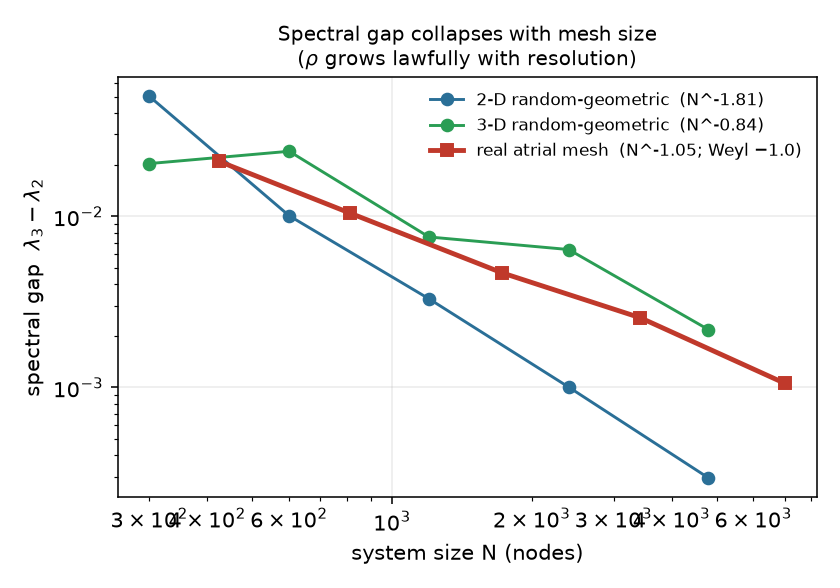
\includegraphics[width=0.82\linewidth]{fig_rho_scaling.png}
\caption{The estimator-validity boundary. The spectral gap collapses with mesh
resolution, so $\rhoval$ grows lawfully and the first-order estimator degrades
\emph{more}, predictably, as the medium is meshed finer.}
\label{fig:rho}
\end{figure}

\begin{figure}[H]
\centering
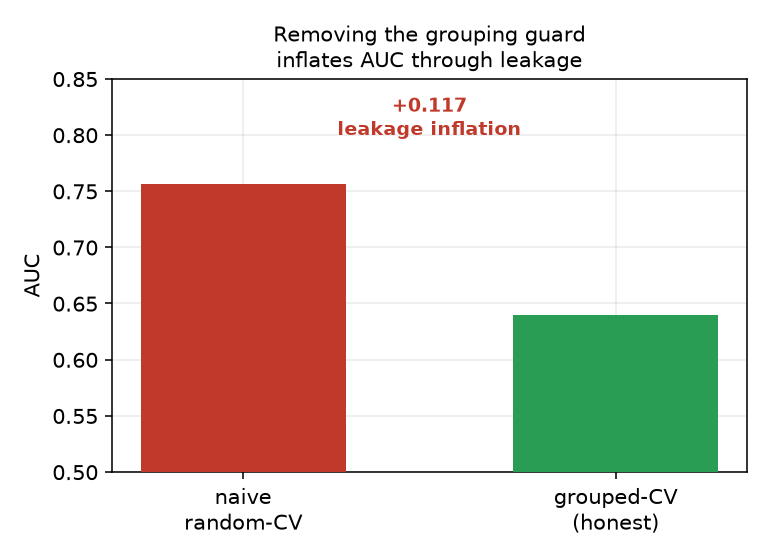
\includegraphics[width=\linewidth]{fig_falsification.png}
\caption{What the pre-registered guards caught. Removing shape-family grouping
inflates AUC by $+0.117$; removing the effect-size gate lets an increment of
$+0.003$ pass at $p=2\times10^{-24}$ on $55{,}000$ networks.}
\label{fig:falsify}
\end{figure}

\end{document}
